\documentclass{article}

\usepackage[final]{neurips_2023}

\usepackage[utf8]{inputenc}
\usepackage[T1]{fontenc}
\usepackage{hyperref}
\usepackage{url}
\usepackage{booktabs}
\usepackage{amsfonts}
\usepackage{nicefrac}
\usepackage{microtype}
\usepackage{xcolor}
\usepackage{graphicx}


\title{Predicting Jet Engine Failure: A Plain Comparison of LSTM and TCN Models on C-MAPSS FD001}


\author{
  Sander Schulman \\
  Department of Mechanical Engineering \\
  Carnegie Mellon University \\
  \texttt{sschulma@andrew.cmu.edu} \\
  \url{https://github.com/sandjman56/deeplearningproject}
}


\begin{document}


\maketitle


\begin{abstract}
We compare an LSTM and a Temporal Convolutional Network (TCN) on the C-MAPSS FD001 turbofan dataset, predicting remaining useful life (RUL) from a window of recent sensor history. Going in, we expected the TCN to win, since recent work reports TCNs matching or beating LSTMs on sequence problems. That is not what we found. The LSTM had a lower error at every window length we tested, and the gap actually grew when we gave both models more history. We argue this happens because FD001 is small, has short windows, and carries a slow smooth degradation signal, which is the kind of regime where LSTMs are usually a better fit.
\end{abstract}


\section{Introduction}

When a jet engine fails in service, the consequences are bad. At best the airline pulls and replaces the engine on an unscheduled timeline, which is expensive. At worst the engine fails in flight, which is dangerous. Airlines and the military both want to know, as accurately as possible, how many more flight cycles a given engine has before something breaks. The standard approach today is a mix of fixed maintenance intervals and human inspection, both of which are conservative by design: engines get pulled well before they would actually fail, which is safe but wasteful. A model that could read recent sensor data and produce a good estimate of remaining useful life (RUL), the number of cycles until failure, would let maintenance planners pull engines closer to their actual wear out point.

NASA released the C-MAPSS dataset in 2008 as a public benchmark for this kind of problem \citep{saxena2008cmapss}. The FD001 subset, which we use here, has 100 simulated training engines and 100 test engines, all run under one operating condition until a single fault mode (high pressure compressor degradation) takes them out. At each cycle, 21 sensors and 3 operating condition variables are recorded. The training engines run to failure; the test engines are cut off at some earlier cycle.

We compare two models on this task. They both consume the same window of recent sensor history; what differs is how they read it. The goal is to figure out which way of reading the data better matches the actual signal in FD001, and to explain why.


\section{Methods}

\paragraph{Data and preprocessing.} For each cycle of each training engine we compute the true RUL by counting forward to the engine's last cycle. Following standard practice for this dataset \citep{zheng2017lstm}, we cap RUL at 125 cycles. The reason is that when an engine is brand new, all the engines look basically the same on the sensors, so trying to tell ``300 cycles left'' from ``280 cycles left'' is mostly fitting noise. Capping at 125 lets the model focus on the part of life where the sensors actually carry signal. We drop the seven sensors and one operating condition variable that are essentially constant across the dataset (training set standard deviation below $10^{-4}$), leaving 17 informative features. Each feature is standardized using only the training mean and standard deviation, so the test set never leaks into preprocessing. We hold out 20 of the 100 training engines as a validation set, used to pick the best epoch for each model. By default each model sees a sliding window of $W{=}30$ cycles; we also sweep $W \in \{15, 30, 50\}$ later.

\paragraph{Baseline (LSTM).} The LSTM is a classic recurrent network: it reads the window one cycle at a time, and at each step it updates a small ``memory'' vector that summarizes everything it has seen so far. The memory at the end of the last cycle is what we use to predict RUL. We use a 2 layer \texttt{nn.LSTM} with hidden size 64 and dropout 0.2, followed by a small ReLU layer and a linear output. This architecture and these hyperparameters follow \citet{zheng2017lstm}, who established the LSTM as a standard baseline for C-MAPSS RUL prediction. The idea is that this kind of running memory should pick up a degradation signal that builds up slowly over time \citep{hochreiter1997lstm}.

\paragraph{Variant (TCN).} The Temporal Convolutional Network \citep{bai2018tcn} does not read the window step by step. Instead, it applies a stack of 1D convolutional filters to the whole window, and each layer's filters are spaced further apart than the last (dilations of 1, 2, 4, 8). Early layers see short patterns and later layers see wider ones, all in one pass instead of one cycle at a time. We use four such layers with kernel size 3 and dropout 0.2, giving a receptive field of 31 cycles, just enough to cover the $W{=}30$ window. We picked the TCN as our variant because Bai et al.\ argue, with strong empirical results on a range of sequence benchmarks, that TCNs should be the default starting point for sequence modeling rather than LSTMs. The structure is similar to WaveNet's dilated convolutions \citep{oord2016wavenet}, which made the same kind of argument in the audio domain.

\paragraph{Training.} Both models are trained with Adam \citep{kingma2015adam} at learning rate $10^{-3}$, batch size 512, mean squared error loss against the capped RUL target. The headline run is 30 epochs at $W{=}30$; the window sweep is 20 epochs per setting. We save the model from the epoch with the lowest validation RMSE and report test set numbers from that checkpoint. The random seed is 0 for both \texttt{numpy} and \texttt{torch}, so the comparison is reproducible. Both models are implemented in PyTorch \citep{paszke2019pytorch}; data loading and preprocessing use NumPy \citep{harris2020numpy} and pandas \citep{mckinney2010pandas}, and figures are generated with Matplotlib \citep{hunter2007matplotlib}. Preprocessing conventions (RUL clipping at 125, dropping near constant sensors, train stat z scoring) follow \citet{zheng2017lstm} and \citet{li2018cmapss_cnn}.


\section{Results and Discussion}

\paragraph{What the metrics mean.} We report two test set numbers. RMSE (root mean squared error) is the typical regression metric: average size of the prediction error in flight cycles. An RMSE of 14 means the model is, on average, off by 14 cycles. The PHM score is the asymmetric scoring function used by the prognostics community \citep{saxena2008cmapss}. It grows exponentially with the error and penalizes \emph{late} predictions (model said 30 cycles left, the engine actually had 10) more steeply than \emph{early} predictions (model said 30, actually had 50). PHM is closer to what an operator actually cares about, since being late is the dangerous mistake.

\paragraph{Headline comparison.} Table~\ref{tab:headline} reports both metrics on the 100 held out test engines at $W{=}30$. The LSTM has a lower RMSE (14.0 vs.\ 16.6 cycles) and a much lower PHM score (601 vs.\ 829), and it does it with about $40\%$ fewer parameters (57k vs.\ 92k). Figure~\ref{fig:curves} shows the training and validation curves: both models reach similar training loss, but the TCN's validation RMSE plateaus higher than the LSTM's. So the TCN is not capacity limited, it just generalizes worse.

\begin{table}[h]
  \caption{Test set performance on FD001 at $W{=}30$.}
  \label{tab:headline}
  \centering
  \begin{tabular}{lrrrr}
    \toprule
    Model & RMSE (capped) & RMSE (uncapped) & PHM score & Params \\
    \midrule
    LSTM (baseline) & \textbf{13.98} & \textbf{15.58} & \textbf{601.4} & 56{,}641 \\
    TCN (variant)   & 16.59 & 17.46 & 829.2 & 91{,}521 \\
    \bottomrule
  \end{tabular}
\end{table}

\begin{figure}[h]
  \centering
  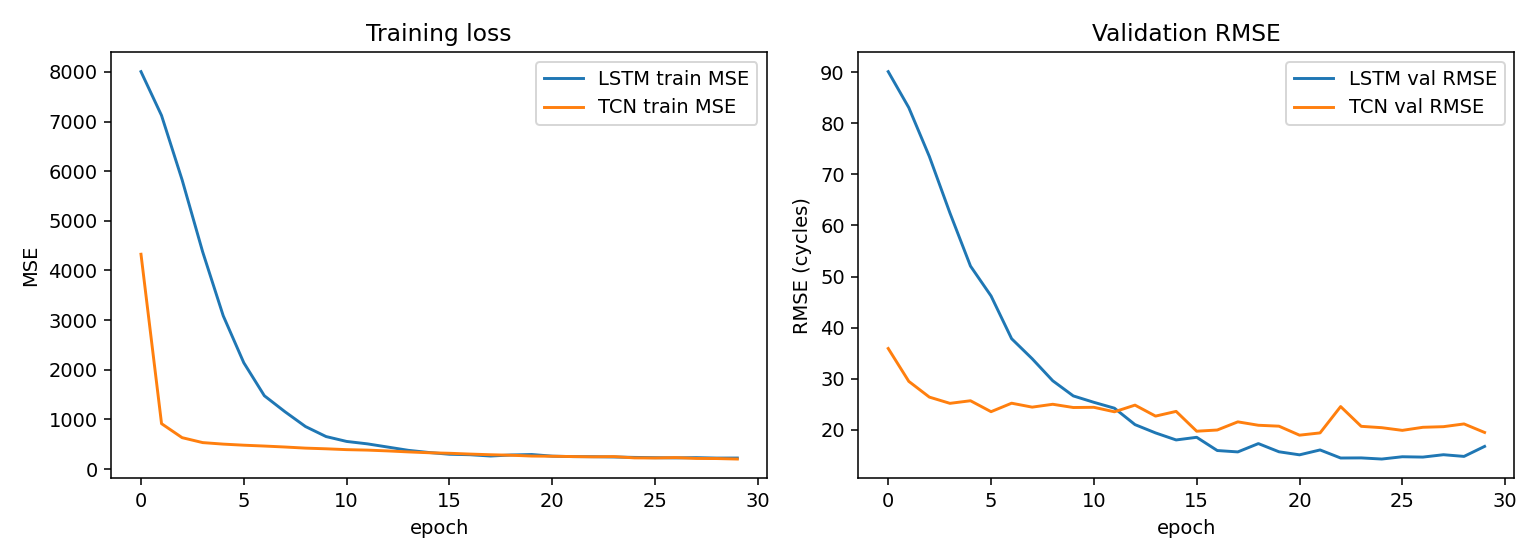
\includegraphics[width=0.85\linewidth]{../figures/training_curves.png}
  \caption{Training MSE (left) and validation RMSE (right) over 30 epochs at $W{=}30$. The TCN's training loss is similar to the LSTM's, but its validation error never gets as low.}
  \label{fig:curves}
\end{figure}

\begin{figure}[h]
  \centering
  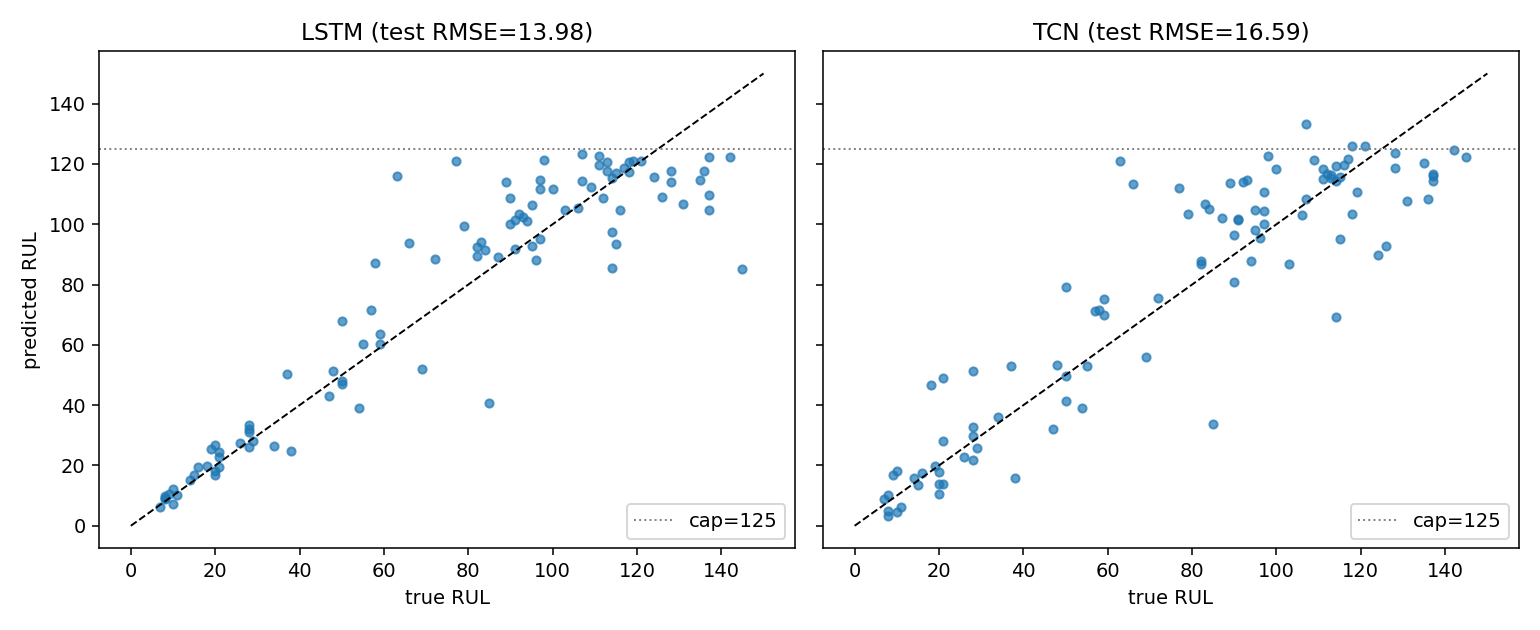
\includegraphics[width=0.85\linewidth]{../figures/pred_vs_true.png}
  \caption{Predicted vs.\ true RUL on the test set at $W{=}30$. Both models compress predictions toward the cap (gray dotted line) for engines with a lot of life left, which is what the cap is supposed to do. The TCN's points scatter more, especially in the 40--80 cycle range.}
  \label{fig:scatter}
\end{figure}

\paragraph{Window length sweep.} Table~\ref{tab:sweep} shows what happens when we vary how much history each model gets: 15, 30, or 50 cycles. The LSTM gets monotonically better at PHM as the window grows (804 to 601 to 448), which is the behavior you would expect from a model that benefits from more context. The TCN gets \emph{worse} on both metrics at $W{=}50$: doubling the window hurts it.

\begin{table}[h]
  \caption{Window length sweep. RMSE is computed against the capped target.}
  \label{tab:sweep}
  \centering
  \begin{tabular}{rrrrr}
    \toprule
    $W$ & LSTM RMSE & TCN RMSE & LSTM PHM & TCN PHM \\
    \midrule
    15 & 16.96 & 17.99 & 804.4 & 1067.6 \\
    30 & \textbf{13.98} & 16.59 & 601.4 & 829.2 \\
    50 & 14.24 & 19.57 & \textbf{448.4} & 1419.8 \\
    \bottomrule
  \end{tabular}
\end{table}

\begin{figure}[h]
  \centering
  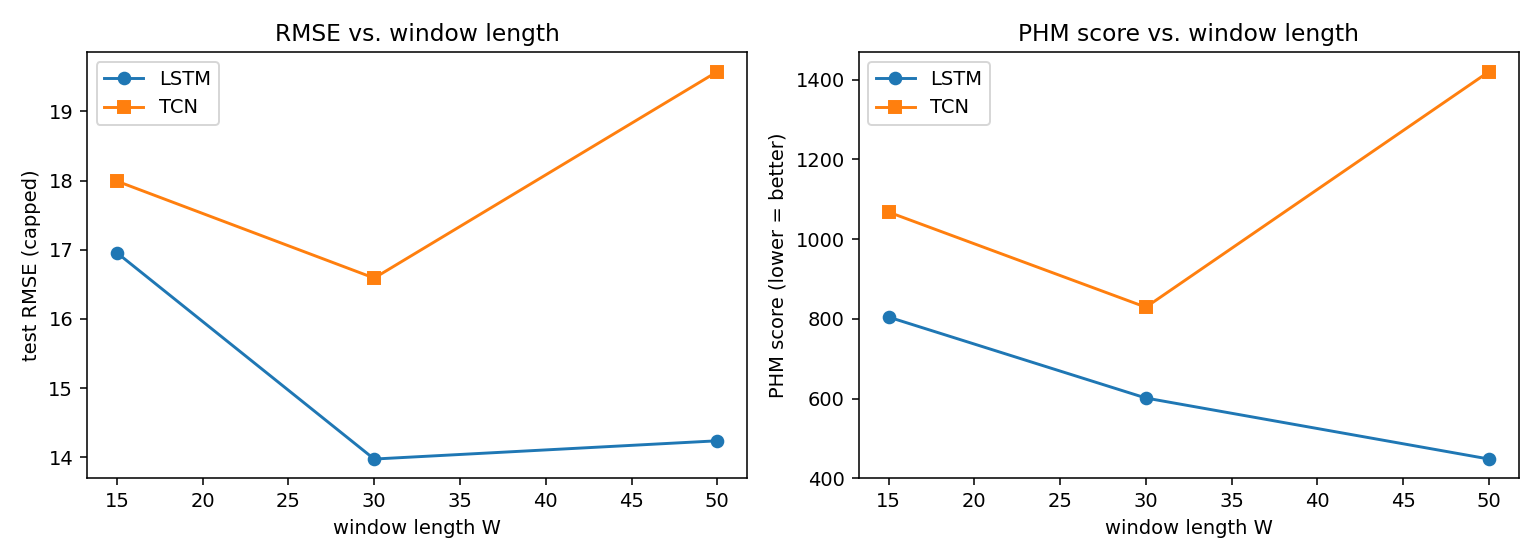
\includegraphics[width=0.85\linewidth]{../figures/window_sweep.png}
  \caption{Test RMSE (left) and PHM score (right) as a function of window length $W$. The LSTM keeps improving on PHM as $W$ grows; the TCN gets worse on both metrics at $W{=}50$, even with more information available.}
  \label{fig:sweep}
\end{figure}

\paragraph{Why the LSTM wins here.} Going in, we expected the TCN to match or beat the LSTM at $W{=}30$ and pull further ahead at $W{=}50$. The data did the opposite. Looking at the literature more carefully after the fact, this is less surprising than it first seemed.

The TCN's advantages over an LSTM are well documented. It trains faster because it can process the whole window at once instead of one cycle after another. It does not suffer from the recurrent network's tendency to forget information from far back in the sequence. Its dilated filters can in principle reach across hundreds or thousands of timesteps. But these advantages mostly help when you have lots of data, long sequences, many input channels, or signals with sharp local patterns or precise long range dependencies. The benchmarks where Bai et al.\ \citep{bai2018tcn} originally showed TCN superiority, like copy memory tasks that require remembering an exact value 1{,}000 steps later or polyphonic music with sharp note onsets, all sit in that regime.

FD001 doesn't. After the validation split, we have about 80 training engines, which is not a lot of data. The window is at most 50 cycles, which is short. There are 17 input features, which is low dimensional. And the actual signal the model has to extract is a slow, near monotonic drift in a handful of sensor channels over the final $\sim$125 cycles of an engine's life. There aren't sharp local patterns to detect, and there isn't a long range exact dependency that has to be preserved. What matters at the end of any window is roughly a smoothed estimate of where the trend is heading.

An LSTM's running memory is well suited for that. As the LSTM sees a longer window, its hidden state has more cycles to integrate over, so it converges on a cleaner trend estimate, which is why its PHM keeps improving from $W{=}15$ to $W{=}50$. The TCN, on the other hand, has 92k parameters and is built around filters that look for local patterns. With only 80 engines and a smooth signal, a lot of that capacity ends up fitting noise. Going from $W{=}30$ to $W{=}50$ gives it more positions in which to overfit, and that lines up with what we see: training loss stays comparable but test PHM nearly doubles, from 829 at $W{=}30$ to 1{,}420 at $W{=}50$.

The parameter counts back this up. The LSTM wins with $40\%$ fewer parameters, which rules out an argument that the TCN just needed more capacity. It also matches the rough ``when to use which'' guidance in comparative reviews: TCNs for large datasets, long sequences, and high dimensional inputs; LSTMs for smaller datasets, shorter sequences, and signals where a recurrent memory makes sense. FD001 falls in the second category. So this isn't really evidence against TCNs in general; it just means FD001 isn't the kind of problem TCNs were built for.

\paragraph{Limitations.} We report a single random seed and a single fault mode (FD001). The result may not transfer to FD002--FD004, which include multiple operating conditions and fault modes. There the data is more heterogeneous and the local feature extractor a TCN provides might genuinely help. We also did not separately tune TCN hyperparameters (channel count, kernel size, dropout); a more aggressive regularization or a smaller TCN might close some of the gap, although we doubt it would flip the ordering.


\section{Conclusion}

On C-MAPSS FD001, a 2 layer LSTM beats a 4 layer dilated TCN at every window length we tested, and the gap widens with more context. This isn't a knock on TCNs in general. The task here just has a small dataset, short windows, low dimensional inputs, and a smooth degradation signal, and that combination is the kind of problem where an LSTM is usually the right pick. The most useful follow up is a multi seed evaluation on FD002 and FD004, where the multi condition / multi fault structure should give a TCN more of what it is good at. A second direction is a hybrid model where a TCN extracts local features and an LSTM summarizes them over time, which is a recommended pattern in comparative reviews and would let each component do what it does best.


\section*{Collaboration Statement}

This is a solo project; all design, implementation, results, and analysis are my own. I used Anthropic's Claude (via Claude Code) as a coding assistant during the project. Specifically, AI assistance was used for: (i)~boilerplate generation of the C-MAPSS download/preprocessing scaffolding, (ii)~the LaTeX skeleton for tables and figures in this report, and (iii)~routine debugging help (e.g., diagnosing a nested zip extraction issue in the data download cell). All architectural choices, the hypothesis, the experimental design including the window sweep, the interpretation of results in Section~3, and the conclusion are my own work. No code or text was lifted from public LLM shared notebooks or third party repositories; the TCN block follows \citet{bai2018tcn} but was implemented from the paper rather than copied.


\bibliographystyle{unsrtnat}
\bibliography{references}


\end{document}
